\ifx\allfiles\undefined
\documentclass[12pt, a4paper, oneside, UTF8]{ctexbook}
\def\path{../../config}
\usepackage{amsmath}
\usepackage{amsthm}
\usepackage{amssymb}
\usepackage{array}
\usepackage{xcolor}
\usepackage{graphicx}
\usepackage{mathrsfs}
\usepackage{enumitem}
\usepackage{geometry}
\usepackage[colorlinks, linkcolor=black]{hyperref}
\usepackage{stackengine}
\usepackage{yhmath}
\usepackage{extarrows}
\usepackage{tikz}
\usepackage{pgfplots}
\usepackage{asymptote}
\usepackage{float}
\usepackage{fontspec} % 使用字体

\setmainfont{Times New Roman}
\setCJKmainfont{LXGWWenKai-Light}[
    SlantedFont=*
]

\everymath{\displaystyle}

\usepgfplotslibrary{polar}
\usepackage{subcaption}
\usetikzlibrary{decorations.pathreplacing, positioning}

\usepgfplotslibrary{fillbetween}
\pgfplotsset{compat=1.18}
% \usepackage{unicode-math}
\usepackage{esint}
\usepackage[most]{tcolorbox}

\usepackage{fancyhdr}
\usepackage[dvipsnames, svgnames]{xcolor}
\usepackage{listings}

\definecolor{mygreen}{rgb}{0,0.6,0}
\definecolor{mygray}{rgb}{0.5,0.5,0.5}
\definecolor{mymauve}{rgb}{0.58,0,0.82}
\definecolor{NavyBlue}{RGB}{0,0,128}
\definecolor{Rhodamine}{RGB}{255,0,255}
\definecolor{PineGreen}{RGB}{0,128,0}

\graphicspath{ {figures/},{../figures/}, {config/}, {../config/} }

\linespread{1.6}

\geometry{
    top=25.4mm, 
    bottom=25.4mm, 
    left=20mm, 
    right=20mm, 
    headheight=2.17cm, 
    headsep=4mm, 
    footskip=12mm
}

\setenumerate[1]{itemsep=5pt,partopsep=0pt,parsep=\parskip,topsep=5pt}
\setitemize[1]{itemsep=5pt,partopsep=0pt,parsep=\parskip,topsep=5pt}
\setdescription{itemsep=5pt,partopsep=0pt,parsep=\parskip,topsep=5pt}

\lstset{
    language=Mathematica,
    basicstyle=\tt,
    breaklines=true,
    keywordstyle=\bfseries\color{NavyBlue}, 
    emphstyle=\bfseries\color{Rhodamine},
    commentstyle=\itshape\color{black!50!white}, 
    stringstyle=\bfseries\color{PineGreen!90!black},
    columns=flexible,
    numbers=left,
    numberstyle=\footnotesize,
    frame=tb,
    breakatwhitespace=false,
} 

\lstset{
    language=TeX, % 设置语言为 TeX
    basicstyle=\ttfamily, % 使用等宽字体
    breaklines=true, % 自动换行
    keywordstyle=\bfseries\color{NavyBlue}, % 关键字样式
    emphstyle=\bfseries\color{Rhodamine}, % 强调样式
    commentstyle=\itshape\color{black!50!white}, % 注释样式
    stringstyle=\bfseries\color{PineGreen!90!black}, % 字符串样式
    columns=flexible, % 列的灵活性
    numbers=left, % 行号在左侧
    numberstyle=\footnotesize, % 行号字体大小
    frame=tb, % 顶部和底部边框
    breakatwhitespace=false % 不在空白处断行
}

% \begin{lstlisting}[language=TeX] ... \end{lstlisting}

% 定理环境设置
\usepackage[strict]{changepage} 
\usepackage{framed}

\definecolor{greenshade}{rgb}{0.90,1,0.92}
\definecolor{redshade}{rgb}{1.00,0.88,0.88}
\definecolor{brownshade}{rgb}{0.99,0.95,0.9}
\definecolor{lilacshade}{rgb}{0.95,0.93,0.98}
\definecolor{orangeshade}{rgb}{1.00,0.88,0.82}
\definecolor{lightblueshade}{rgb}{0.8,0.92,1}
\definecolor{purple}{rgb}{0.81,0.85,1}

\theoremstyle{definition}
\newtheorem{myDefn}{\indent Definition}[section]
\newtheorem{myLemma}{\indent Lemma}[section]
\newtheorem{myThm}[myLemma]{\indent Theorem}
\newtheorem{myCorollary}[myLemma]{\indent Corollary}
\newtheorem{myCriterion}[myLemma]{\indent Criterion}
\newtheorem*{myRemark}{\indent Remark}
\newtheorem{myProposition}{\indent Proposition}[section]

\newenvironment{formal}[2][]{%
	\def\FrameCommand{%
		\hspace{1pt}%
		{\color{#1}\vrule width 2pt}%
		{\color{#2}\vrule width 4pt}%
		\colorbox{#2}%
	}%
	\MakeFramed{\advance\hsize-\width\FrameRestore}%
	\noindent\hspace{-4.55pt}%
	\begin{adjustwidth}{}{7pt}\vspace{2pt}\vspace{2pt}}{%
		\vspace{2pt}\end{adjustwidth}\endMakeFramed%
}

\newenvironment{definition}{\vspace{-\baselineskip * 2 / 3}%
	\begin{formal}[Green]{greenshade}\vspace{-\baselineskip * 4 / 5}\begin{myDefn}}
	{\end{myDefn}\end{formal}\vspace{-\baselineskip * 2 / 3}}

\newenvironment{theorem}{\vspace{-\baselineskip * 2 / 3}%
	\begin{formal}[LightSkyBlue]{lightblueshade}\vspace{-\baselineskip * 4 / 5}\begin{myThm}}%
	{\end{myThm}\end{formal}\vspace{-\baselineskip * 2 / 3}}

\newenvironment{lemma}{\vspace{-\baselineskip * 2 / 3}%
	\begin{formal}[Plum]{lilacshade}\vspace{-\baselineskip * 4 / 5}\begin{myLemma}}%
	{\end{myLemma}\end{formal}\vspace{-\baselineskip * 2 / 3}}

\newenvironment{corollary}{\vspace{-\baselineskip * 2 / 3}%
	\begin{formal}[BurlyWood]{brownshade}\vspace{-\baselineskip * 4 / 5}\begin{myCorollary}}%
	{\end{myCorollary}\end{formal}\vspace{-\baselineskip * 2 / 3}}

\newenvironment{criterion}{\vspace{-\baselineskip * 2 / 3}%
	\begin{formal}[DarkOrange]{orangeshade}\vspace{-\baselineskip * 4 / 5}\begin{myCriterion}}%
	{\end{myCriterion}\end{formal}\vspace{-\baselineskip * 2 / 3}}
	

\newenvironment{remark}{\vspace{-\baselineskip * 2 / 3}%
	\begin{formal}[LightCoral]{redshade}\vspace{-\baselineskip * 4 / 5}\begin{myRemark}}%
	{\end{myRemark}\end{formal}\vspace{-\baselineskip * 2 / 3}}

\newenvironment{proposition}{\vspace{-\baselineskip * 2 / 3}%
	\begin{formal}[RoyalPurple]{purple}\vspace{-\baselineskip * 4 / 5}\begin{myProposition}}%
	{\end{myProposition}\end{formal}\vspace{-\baselineskip * 2 / 3}}


\newtheorem{example}{\indent \color{SeaGreen}{Example}}[section]
\renewcommand{\proofname}{\indent\textbf{\textcolor{TealBlue}{Proof}}}
\NewEnviron{solution}{%
	\begin{proof}[\indent\textbf{\textcolor{TealBlue}{Solution}}]%
		\color{blue}% 设置内容为蓝色
		\BODY% 插入环境内容
		\color{black}% 恢复默认颜色(可选,避免影响后续文字)
	\end{proof}%
}

% 自定义命令的文件

\def\d{\mathrm{d}}
\def\R{\mathbb{R}}
%\newcommand{\bs}[1]{\boldsymbol{#1}}
%\newcommand{\ora}[1]{\overrightarrow{#1}}
\newcommand{\myspace}[1]{\par\vspace{#1\baselineskip}}
\newcommand{\xrowht}[2][0]{\addstackgap[.5\dimexpr#2\relax]{\vphantom{#1}}}
\newenvironment{mycases}[1][1]{\linespread{#1} \selectfont \begin{cases}}{\end{cases}}
\newenvironment{myvmatrix}[1][1]{\linespread{#1} \selectfont \begin{vmatrix}}{\end{vmatrix}}
\newcommand{\tabincell}[2]{\begin{tabular}{@{}#1@{}}#2\end{tabular}}
\newcommand{\pll}{\kern 0.56em/\kern -0.8em /\kern 0.56em}
\newcommand{\dive}[1][F]{\mathrm{div}\;\boldsymbol{#1}}
\newcommand{\rotn}[1][A]{\mathrm{rot}\;\boldsymbol{#1}}

\newif\ifshowanswers
\showanswerstrue % 注释掉这行就不显示答案

% 定义答案环境
\newcommand{\answer}[1]{%
    \ifshowanswers
        #1%
    \fi
}

% 修改参数改变封面样式,0 默认原始封面、内置其他1、2、3种封面样式
\def\myIndex{0}


\ifnum\myIndex>0
    \input{\path/cover_package_\myIndex} 
\fi

\def\myTitle{考研数学笔记}
\def\myAuthor{Weary Bird}
\def\myDateCover{\today}
\def\myDateForeword{\today}
\def\myForeword{相见欢·林花谢了春红}
\def\myForewordText{
    林花谢了春红,太匆匆。
    无奈朝来寒雨晚来风。
    胭脂泪,相留醉,几时重。
    自是人生长恨水长东。
}
\def\mySubheading{以姜晓千强化课讲义为底本}



\begin{document}
% \input{\path/cover_text_\myIndex.tex}

\newpage
\thispagestyle{empty}
\begin{center}
    \Huge\textbf{\myForeword}
\end{center}
\myForewordText
\begin{flushright}
    \begin{tabular}{c}
        \myDateForeword
    \end{tabular}
\end{flushright}

\newpage
\pagestyle{plain}
\setcounter{page}{1}
\pagenumbering{Roman}
\tableofcontents

\newpage
\pagenumbering{arabic}
% \setcounter{chapter}{-1}
\setcounter{page}{1}

\pagestyle{fancy}
\fancyfoot[C]{\thepage}
\renewcommand{\headrulewidth}{0.4pt}
\renewcommand{\footrulewidth}{0pt}








\else
\fi
\chapter{二维随机变量}

\section{联合分布函数的计算}
\begin{remark}
    (联合分布函数的性质)
    \item[(1)] $0\leq F(x,y)\leq 1,-\infty<x<+\infty, F(-\infty,y)=F(x,-\infty)=F(-\infty,-\infty)=0,F(+\infty,+\infty)=1$
    \item[(2)] $F(x,y)$关于$x$和$y$均单调不减
    \item[(2)] $F(x,y)$关于$x$和$y$均右连续
    \item[(4)] $P\{a<X\leq b,c<Y\leq b\}=F(b,d)-F(b,c)-F(a,d)+F(a,c)$  
\end{remark}

\begin{enumerate}[label=\arabic*.]
    % 例题3.1
    \item 设随机变量$X$与$Y$相互独立,$X\sim B(1,p)$,$Y\sim E(\lambda)$,则$(X,Y)$的联合分布函数$F(x,y)=$\_\_\_.
    
    \begin{solution}
    由$X$和$Y$相互独立,则有$F_{XY}(x,y)=F_{X}(x)F_{Y}(y),f(x,y)=f_{X}(x)F_{Y}(x)$,$X$的概率分布如下:
    \[
    \begin{array}{c|c|c}
        X&0&1\\
        P&1-p&p
    \end{array}
    \]
    则$X$的分布函数为
    \[F_{X}(x)=
    \begin{cases}
        0, & x < 0\\
        1-p, & 0\leq x < 1\\
        1, &x\geq 1
    \end{cases}
    \]
    而$Y\sim E(\lambda)$,故
    \[
    F_{XY}(x,y)=F_{X}(x)F_{Y}(y)=\begin{cases}
        (1-p)(1-e^{-\lambda y}), & 0\leq x < 1,\, y > 0 \\
        1-e^{-\lambda y}, & x\geq 1,\, y > 0\\
        0, & \text{其他}
    \end{cases}
    \]
    \end{solution}
\end{enumerate}

\section{二维离散型随机变量分布的计算}

\begin{enumerate}[label=\arabic*.,start=2]
    % 例题3.2
    \item 设随机变量$X$与$Y$相互独立,均服从参数为$p$的几何分布。
    \begin{enumerate}
        \item 求在$X+Y=n(n\geq 2)$的条件下,$X$的条件概率分布;
        \item 求$P\{X+Y\geq n\}(n\geq 2)$.
    \end{enumerate}
    
    \begin{solution}
    \item {(1)} 
    \begin{align*}
        P\{X+Y=n\} &\xlongequal{\text{几何分布从1开始}}\sum_{k=1}^{n-1}P\{X=k, Y=n-k\} \\
        &\xlongequal{\text{独立性}}\sum_{k=1}^{n-1}P\{X=k\}P\{Y=n-k\} \\
        &=\sum_{k=1}^{n-1}(1-p)^{k-1}p\cdot(1-p)^{n-k-1}p \\
        &=\sum_{k=1}^{n-1}(1-p)^{n-2}p^2 \\
        &=(n-1)(1-p)^{n-2}p^2
    \end{align*}
    在$X+Y=n$的条件下,$X$的条件概率为
    \begin{align*}
        P\{X=k\mid X+Y=n\} &= \frac{P\{X=k,Y=n-k\}}{P\{X+Y=n\}} \\
        &=\frac{p^2(1-p)^{n-2}}{(n-1)p^2(1-p)^{n-2}} \\
        &=\frac{1}{n-2} \\ 
        &{\color{red}k=1,2\ldots n - 1} \text{这个范围千万别忘喽!}
    \end{align*}
    \item [(2)]
    \begin{align*}
        P\{X+Y\geq n\} &= P\{X+Y=n\} + P\{X+Y=n+1\} + \ldots \\
        &=\sum_{k=n}^{+\infty}P\{X+Y=k\} \\
        &=\sum_{k=n}^{+\infty}(k-1)p^2(1-p)^{k-2} \\
    \end{align*}
    不妨先计算级数$\sum_{k=n}^{\infty}(k-1)x^{k-2}$ 
    \begin{align*}
        \sum_{k=n}^{\infty}(k-1)x^{k-2}
        &= \sum_{k=n}^{\infty}(x^{k-1})' \\
        &= \left(\frac{\sum_{n=k}^{\infty}}{x}\right)' \\
        &=\frac{(n-1)x^{n-2}(1-x)+x^{n-1}}{(1-x)^2}
    \end{align*}
    故当$x=1-p$的时有\begin{align*}
        P\{X+Y\geq n\} &= p^2 \frac{(n-1)(1-p)^{n-2}p+(1-p)^{n-1}}{p^2} \\
        &=(1-p)^{n-2}(np-2p+1)
    \end{align*}
    \end{solution}
\end{enumerate}

\section{二维连续型随机变量分布的计算}
\begin{remark}
\begin{enumerate} 主要内容 \\
联合概率密度的性质
    \item [(1)] $f\left( {x,y}\right)  \geq  0, - \infty  < x <  + \infty , - \infty  < y <  + \infty$ ;
    \item [(2)] ${\int }_{-\infty }^{+\infty }{\int }_{-\infty }^{+\infty }f\left( {x,y}\right) {dxdy} = 1$ ;
    \item [(3)] $P\{ \left( {X,Y}\right)  \in  D\}  = {\iint }_{D}f\left( {x,y}\right) {dxdy}$ ;
    \item [(4)]在 $f\left( {x,y}\right)$ 的连续点处有 $\frac{{\partial }^{2}F\left( {x,y}\right) }{\partial x\partial y} = f\left( {x,y}\right)$ .\\
边缘概率密度
    \item[(1)](X,Y)关于 $X$ 的边缘概率密度 ${f}_{X}\left( x\right)  = {\int }_{-\infty }^{+\infty }f\left( {x,y}\right) {dy}$
    \item[(2)](X,Y)关于 $Y$ 的边缘概率密度 ${f}_{Y}\left( y\right)  = {\int }_{-\infty }^{+\infty }f\left( {x,y}\right) {dx}$\\
条件概率密度
    \item[(1)]在 $Y = y$ 的条件下, $X$ 的条件概率密度 ${f}_{X \mid  Y}\left( {x \mid  y}\right)  = \frac{f\left( {x,y}\right) }{{f}_{Y}\left( y\right) }$
    \item[(2)]在 $X = x$ 的条件下, $Y$ 的条件概率密度 ${f}_{Y \mid  X}\left( {y \mid  x}\right)  = \frac{f\left( {x,y}\right) }{{f}_{X}\left( x\right) }$
\end{enumerate}
\end{remark}
\begin{enumerate}[label=\arabic*.,start=3]
    % 例题3.3
    \item (2010,数一、三)设二维随机变量$(X,Y)$的概率密度为
    \begin{align*}
        f(x,y)=Ae^{-2x^2+2xy-y^2}, \quad -\infty<x<+\infty, -\infty<y<+\infty
    \end{align*}
    求常数$A$及条件概率密度$f_{Y|X}(y|x)$.
    
    \begin{solution}
    \item [(方法一 正常求)]
    首先通过规范性求出参数A\begin{align*}
        \int_{-\infty}^{+\infty}\int_{-\infty}^{+\infty}f(x,y)\d x\d y &=
        \int_{-\infty}^{+\infty}\int_{-\infty}^{+\infty}Ae^{-2x^2+2xy-y^2}\d x\d y \\
        &=A\int_{-\infty}^{+\infty}e^{-x^2}\d x\int_{-\infty}^{+\infty} e^{-(y-x)^2}\d y\\
        &\xlongequal{\text{Possion积分}} A\pi = 1 \implies A=\frac{1}{\pi}
    \end{align*}
    $X$的边缘分布函数为
    \begin{align*}
        \int_{-\infty}^{+\infty}f(x,y)dy &=\int_{-\infty}^{+\infty}\frac{1}{\pi}e^{-2x^2+2xy-y^2}\d y\\
        &=\frac{1}{\pi}e^{-x^2}\int_{-\infty}^{+\infty}e^{-(y-x)^2} \\
        &=\frac{1}{\sqrt{\pi}}e^{-x^2}, x\in \mathbf{R}
    \end{align*}
    则在$X=x$的条件下,$Y$的条件概率为
    \begin{align*}
        f_{Y\mid X}(y\mid x) &=\frac{f(x,y)}{f_{X}(x)}  \\
        &= \frac{1}{\sqrt{\pi}}e^{-(y-x)^2}
    \end{align*}
    \item [(方法二,通过二维正态分布)]
    形如$f(x,y)=Ae^{ax^2+bxy+cy^2}$的函数如果是概率密度,则其一定是某个二维正态的概率密度函数,故
    \[
    (X,Y)\sim N(\mu_1,\mu_2;\sigma_1^2,\sigma_2^2;\rho)
    \]
    通过下一节讲的确定系数的办法,可以很快的确定
    \[
    (X,Y)\sim N(0,0;\frac{1}{2},1;\frac{\sqrt{2}}{2})
    \]
    故$A=\frac{1}{2\pi\sigma_1\sigma_2\sqrt{1-\rho^2}}=\frac{1}{\pi},
    f_{X}(x)=\frac{1}{\sqrt{\pi}}e^{-x^2}$
    \end{solution}
    
    % 例题3.4
    \item 设随机变量$X\sim U(0,1)$,在$X=x(0<x<1)$的条件下,随机变量$Y\sim U(x,1)$。
    \begin{enumerate}
        \item 求$(X,Y)$的联合概率密度;
        \item 求$(X,Y)$关于$Y$的边缘概率密度$f_Y(y)$;
        \item 求$P\{X+Y>1\}$.
    \end{enumerate}
    
    \begin{solution}
    \item [(1)]
    在$X=x$的条件下,$Y$的条件概率密度为
    \[
    f_{Y}(y)=\begin{cases}
        \frac{1}{1-x}, &x\leq y\leq 1 \\
        0, &\text{其他}
    \end{cases}
    \]
    故$f(x,y)=f_{Y\mid X}(y\mid x)f_{X}(x)=\begin{cases}
        \frac{1}{1-x}, &0 < x < 1, x < y < 1 \\
        0, &\text{其他}
    \end{cases}$
    \item [(2)]
    通过概率密度求边缘密度的时候,需要画出x-y图,并且确定要求的那个参数的范围,比如说这里是$y\in (0,1)$,让后再
    从[0,1]上面去做偏积分,具体如图所示
    \begin{center}
        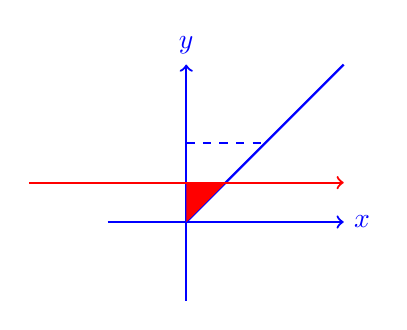
\begin{tikzpicture}
        \draw[blue, thick, ->] (-1,0) -- (2,0) node[right] {$x$};
        \draw[blue, thick, ->] (0,-1) -- (0,2) node[above] {$y$};
        \draw[blue, thick](0,0) -- (2,2);
        \draw[blue, thick,dashed](0,1) -- (1,1);
        \draw[red, thick, ->](-2, 0.5) -- (2,0.5);
        \fill[red](0,0.5)--(0.5,0.5)--(0,0);
    \end{tikzpicture}
    \end{center}
    $f_{Y}(y)=\int_{+\infty}^{-\infty}f(x,y)\d x=\begin{cases}
        -\ln{(1-y)}, &0< y < 1 \\
        0, &\text{其他}
    \end{cases}$
    \item [(3)]
    根据性质(3)有$P\{X+Y> 1\} =\iint\limits_{x+y<1}f(x,y)\d x\d y$此时x-y的可行范围为
    \begin{center}
        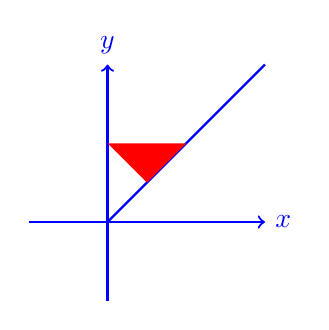
\begin{tikzpicture}
        \draw[blue, thick, ->] (-1,0) -- (2,0) node[right] {$x$};
        \draw[blue, thick, ->] (0,-1) -- (0,2) node[above] {$y$};
        \draw[blue, thick](0,0) -- (2,2);
        \fill[red](0,1)--(1,1)--(0.5,0.5);
    \end{tikzpicture}
    \end{center}
    \begin{align*}
        \text{原式} &= \int_{1/2}^{1} \d y \int_{1-y}^{y} \frac{1}{1-x} \d x \\
        &= \int_{1/2}^{1} \left[ \ln y - \ln(1-y) \right] \d y \\
        &= \left[ y\ln y - (1-y)\ln(1-y) \right] \Big|_{1/2}^{1} \\
        &= \ln 2
    \end{align*}
    \end{solution}
    \section {关于二维正态分布}
    \begin{remark}
        二维正态分布的性质\qquad 设$(X,Y)\sim N(\mu_1,\mu_2;\sigma_1^2,\sigma_2^2;\rho)$,则
        \item[(1)] $X \sim  N\left( {{\mu }_{1},{\sigma }_{1}^{2}}\right) ,Y \sim  N\left( {{\mu }_{2},{\sigma }_{2}^{2}}\right)$ ,反之不成立(独立的时候反之成立);
        \item[(2)] $X$ 与 $Y$ 相互独立 $\Leftrightarrow  X$ 与 $Y$ 不相关 $\left( {\rho  = 0}\right)$ ;
        \item[(3)] ${aX} + {bY} \sim  N\left( {a{\mu }_{1} + b{\mu }_{2},{a}^{2}{\sigma }_{1}^{2} + {b}^{2}{\sigma }_{2}^{2} + {2ab\rho }{\sigma }_{1}{\sigma }_{2}}\right)$;
        特别地,若 $X$ 与 $Y$ 相互独立, $X \sim  N\left( {{\mu }_{1},{\sigma }_{1}^{2}}\right) ,Y \sim  N\left( {{\mu }_{2},{\sigma }_{2}^{2}}\right)$ ,则
        ${aX} + {bY} \sim  N\left( {a{\mu }_{1} + b{\mu }_{2},{a}^{2}{\sigma }_{1}^{2} + {b}^{2}{\sigma }_{2}^{2}}\right) ;$
        \item[(4)]若 $U = {aX} + {bY},V = {cX} + {dY}$ ,即 $\left( \begin{array}{l} U \\  V \end{array}\right)  = \left( \begin{array}{ll} a & b \\  c & d \end{array}\right) \left( \begin{array}{l} X \\  Y \end{array}\right)$ ,则(U,V)服从二维正态分布
        $\Leftrightarrow  \left| \begin{array}{ll} a & b \\  c & d \end{array}\right|  \neq  0$ .
    \end{remark}
    % 例题3.5
    \item 设二维随机变量$(X,Y)\sim N(1,2;1,4;-\frac{1}{2})$,且$P\{aX+bY\leq 1\}=\frac{1}{2}$,则$(a,b)$可以为
    \begin{align*}
        (A)\ \left(\frac{1}{2},-\frac{1}{4}\right) \quad (B)\ \left(\frac{1}{4},-\frac{1}{2}\right)\ 
        (C)\ \left(-\frac{1}{4},\frac{1}{2}\right) \quad (D)\ \left(\frac{1}{2},\frac{1}{4}\right)
    \end{align*}
    
    \begin{solution}
    由性质(3)可知$aX+bY\sim N$,而由正态分布的对称性可知,$\mu=1\implies a+2b=1$故选择$(D)$ 
    \end{solution}
    
    % 例题3.6
    \item (2020,数三)设二维随机变量$(X,Y)\sim N(0,0;1,4;-\frac{1}{2})$,则下列随机变量服从标准正态分布且与$X$相互独立的是
    \begin{align*}
        (A)\ \frac{\sqrt{5}}{5}(X+Y) \quad (B)\ \frac{\sqrt{5}}{5}(X-Y) \ 
        (C)\ \frac{\sqrt{3}}{3}(X+Y) \quad (D)\ \frac{\sqrt{3}}{3}(X-Y)
    \end{align*}
    
    \begin{solution}
    这道题选择出来并不困难,但要证明其与$X$相互独立还是有点说法的.\\
    第一步,先求$X+Y$和$X-Y$的标准化\\
    由性质三可知$X+Y\sim N(0,3), X-Y\sim N(0,7)$,故
    $\frac{\sqrt{3}}{3}(X+Y)\sin N(0,1); \frac{\sqrt{7}}{7}\sim N(0,1)$;这里其时就已经可以选出答案喽 \\
    第二步证明独立性
    \\考虑$(X+Y, X)=\begin{pmatrix}
        1 & 1 \\
        1 & 0 
    \end{pmatrix}\begin{pmatrix}
        X\\
        Y
    \end{pmatrix}$,且$\begin{vmatrix}
        1 & 1\\
        1 & 0
    \end{vmatrix}=-1\neq 0$ \\
    由性质(4)可知,$(X+Y,X)$服从二维正态分布,由性质(2)可知,只需要证明二者的相关系数为0即可,证明二者独立.\\

    \end{solution}
    % 例题3.7
    \item (2022,数一)设随机变量$X\sim N(0,1)$,在$X=x$的条件下,随机变量$Y\sim N(x,1)$,则$X$与$Y$的相关系数为
    \begin{align*}
        (A)\ \frac{1}{4} \quad (B)\ \frac{1}{2} \quad (C)\ \frac{\sqrt{3}}{3} \quad (D)\ \frac{\sqrt{2}}{2}
    \end{align*}
    
    \begin{solution}
    \item[(方法一 传统方法计算)]
    \[
    \rho_{XY}=\frac{Cov(X,Y)}{\sqrt{DX}\sqrt{DY}}=\frac{EXY-EXEY}{\sqrt{DX}\sqrt{DY}}
    \]
    问题转换为求$EXY,DY$,由题设可知,在$X=x$的条件下,$Y$的概率密度函数为
    \[
    f_{Y\mid X}(y\mid x)=\frac{1}{\sqrt{2\pi}}e^{-\frac{(y-x)^2}{2}} 
    \]
    故$(X,Y)$的概率密度函数为
    \[
    f(x,y)=\frac{1}{2\pi}e^{-x^2+xy-\frac{y^2}{2}}
    \]
    故$y$的边缘分布函数为
    \[
    \int_{+\infty}^{-\infty}f(x,y)dx=\frac{1}{2\sqrt{\pi}}e^{-\frac{y^2}{4}}
    \]
    即$Y\sim N(0, 2)$,故$EY=0,DY=2$
    而$EXY$根据方差的定义可以计算 \\
    TODO: 计算EXY
    \begin{align*}
        EXY=\int_{+\infty}^{-\infty}\int_{+\infty}^{-\infty}xyf(x,y)\d x\d y 
        = 1
    \end{align*}
    故$\rho=\frac{\sqrt{2}}{2}$
    \item [(2)]通过二维正态参数的结论直接求出$\rho$, 由上述可知$f(x,y)=\frac{1}{2\pi}
    e^{-x^2+xy-\frac{y^2}{2}}$,对比二维正态概率密度的公式
    \[
    f(x,y)=\frac{1}{2\sigma_1\sigma_2\sqrt{1-\rho^2}}exp\{\frac{-1}{2(1-\rho^2)}\left[
        \frac{(x_1-\mu_1)^2}{\sigma_1^2}-\frac{2(x_1-\mu_1)(x_2-\mu_2)}{\sigma_1\sigma_2}+\frac{(x_2-\mu_2)}{\sigma_2^2}
    \right]\}
    \]
    容易得出$(X,Y)\sim N(0,0;1,2;\frac{\sqrt{2}}{2})$,具体如总结所示.
    \end{solution}
\end{enumerate}
\begin{tcolorbox}[title=总结]
对于形如$Ae^{-ax^2+bxy+cy^2}$的式子,若其是概率密度,则必然是某个二维正态的概率密度(由规范性)且满足
\begin{enumerate}
    \item [(1)] $b^2=4\rho^2a^2c^2\implies \rho^2=\frac{b^2}{4a^2c^2}$
    \item [(2)] $rho$的符号与$xy$系数的符号一致
\end{enumerate}
\end{tcolorbox}
\newpage
\section{求二维离散型随机变量函数的分布}
\begin{enumerate}[label=\arabic*.,start=8]
    % 例题3.8
    \item 设随机变量$X$与$Y$相互独立,$X\sim P(\lambda_1)$,$Y\sim P(\lambda_2)$,求$Z=X+Y$的概率分布.
    
    \begin{solution}
    这道题是参数可加性的直接考察,可以先证明一下
    \begin{align*}
        P\{Z=n\} &= P\{X+Y=n\} \\ 
        &=\sum_{k=0}^{n}P\{X=k, Y=n-k\} \\
        &\xlongequal{\text{独立性}}\sum_{k=0}^{n}P\{X=k\}P\{Y=n-k\}\\
        &=\sum_{k=0}^{n}\frac{\lambda_1^k}{k!}e^{-\lambda_1}\frac{\lambda_2^{n-k}}{(n-k)!}e^{-\lambda_2} \\
        &=e^{-(\lambda_1+\lambda_2)}\sum_{k=0}^{n}\frac{\lambda_1^k\lambda_2^{n-k}}{k!(n-k)!} \\
        &\xlongequal{\text{上下同乘}k!}e^{-(\lambda_1+\lambda_2)}\sum_{k=0}^{n}\frac{n(n-1)\ldots(n-k+1)}{k!}\lambda_1^k\lambda_2^{n-k} \\
        &=e^{-(\lambda_1+\lambda_2)}\frac{1}{n!}\sum_{k=0}^{n}C_{n}^k\lambda_1^k\lambda_2^{n-k} \\
        &\xlongequal{\text{二项式定理}}\frac{(\lambda_1+\lambda_2)^n}{n!}e^{-(\lambda_1+\lambda_2)}
    \end{align*}
    \end{solution}
\end{enumerate}
\begin{tcolorbox}[title=参数可加性]
    当$X,Y$独立的时候
    \begin{enumerate}
        \item [(1)] $X\sim B(m,p), Y\sim B(n,p)\implies X+Y\sim B(n+m, p)$ 
        \item [(2)] $X\sim P(\lambda_1), Y\sim P(\lambda_2)\implies X+Y\sim P(\lambda_1+\lambda_2)$
        \item [(3)] $X\sim N(\mu_1,\sigma_1^2), Y\sim N(\mu_2,\sigma_2^2)\implies X+Y\sim (\mu_1+\mu_2,\sigma_1^2+\sigma_2^2)$
        \item [(4)] $X\sim \chi^2(m), Y\sim \chi^2(n),\implies X+Y\sim \chi^2(n+m)$
        \item [(5)] $X\sim E(\lambda_1), Y\sim E(\lambda_2)\implies \min{(X,Y)}\sim E(\lambda_1+\lambda_2)$
    \end{enumerate}
\end{tcolorbox}
\section{求二维连续型随机变量函数的分布}
\begin{remark}
\textbf{问题描述}\\
设二维随机变量(X,Y)的联合概率密度为 $f\left( {x,y}\right)$ ,
求 $Z = g\left( {X,Y}\right)$ 的概率密度 ${f}_{Z}\left( z\right)$ .\\
\textbf{分布函数法} \\
(1)设 $Z$ 的分布函数为 ${F}_{Z}\left( z\right)$ ,则 ${F}_{Z}\left( z\right)  = P\{ Z \leq  z\}  = P\{ g\left( {X,Y}\right)  \leq  z\}$ .\\
(2)求 $Z = g\left( {X,Y}\right)$ 在(X,Y)的正概率密度区域的值域 $\left( {\alpha ,\beta }\right)$ ,讨论 $z$ .\\
$z < \alpha$ 时, ${F}_{Z}\left( z\right)  = 0$ ; \\
当 $\alpha  \leq  z < \beta$ 时, ${F}_{Z}\left( z\right)  = {\iint }_{g\left( {x,y}\right)  \leq  z}f\left( {x,y}\right) {dxdy}$; \\
当 $z \geq  \beta$ 时, ${F}_{Z}\left( z\right)  = 1$ .\\
(3) $Z$ 的概率密度为 ${f}_{Z}\left( z\right)  = {F}_{Z}^{\prime }\left( z\right)$ . \\
\textbf{卷积公式}\\
(1)设 $Z = {aX} + {bY}$ ,则 
${f}_{Z}\left( z\right)  = {\int }_{-\infty }^{+\infty }\frac{1}{\left| b\right| }f\left( {x,\frac{z - {ax}}{b}}\right) {dx} = {\int }_{-\infty }^{+\infty }\frac{1}{\left| a\right| }f\left( {\frac{z - {by}}{a},y}\right) {dy}$; \\
(2)设 $Z = {XY}$ ,则 
${f}_{Z}\left( z\right)  = {\int }_{-\infty }^{+\infty }\frac{1}{\left| x\right| }f\left( {x,\frac{z}{x}}\right) {dx} = {\int }_{-\infty }^{+\infty }\frac{1}{\left| y\right| }f\left( {\frac{z}{y},y}\right) {dy}$ ; \\
(3)设 $Z = \frac{Y}{X}$ ,
则 ${f}_{Z}\left( z\right)={\int}_{-\infty}^{+\infty}\left|x\right|f\left({x,{xz}}\right){dx}$; \\
(4)设$Z=\frac{X}{Y}$,则${f}_{Z}\left(z\right)={\int}_{-\infty}^{+\infty}\left|y\right|f\left({{yz},y}\right){dy}$ 
\end{remark}
\begin{enumerate}[label=\arabic*.,start=9]
    % 例题3.9
    \item 设二维随机变量$(X,Y)$的联合概率密度为
        $f(x,y)=\begin{cases}
            1, & 0<x<1,0<y<2x \\
            0, & \text{其他}
        \end{cases}$
    求:
    \begin{enumerate}
        \item $(X,Y)$的联合分布函数$F(x,y)$;
        \item $(X,Y)$的边缘概率密度$f_X(x),f_Y(y)$;
        \item 条件概率密度$f_{X|Y}(x|y),f_{Y|X}(y|x)$;
        \item $P\left\{Y\leq \frac{1}{2}|X\leq \frac{1}{2}\right\}$,$P\left\{Y\leq \frac{1}{2}|X=\frac{1}{2}\right\}$;
        \item $Z=2X-Y$的概率密度$f_Z(z)$.
    \end{enumerate}
    \newpage
    \begin{figure}
    \centering
    \begin{subfigure}{0.18\textwidth} % 每个子图约占 18% 的文本宽度,5个加起来略小于1,留出间距
        \centering
        % 概率为零的区域
        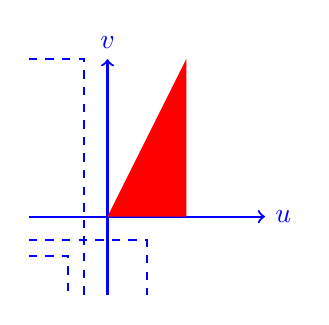
\begin{tikzpicture}
            \draw[blue, thick, ->] (-1,0) -- (2,0) node[right] {$u$};
            \draw[blue, thick, ->] (0,-1) -- (0,2) node[above] {$v$};
            \fill[red] (0,0) -- (1,0) -- (1,2);
            \draw[blue, thick, dashed] (-1,-0.5)--(-0.5,-0.5)--(-0.5,-1);
            \draw[blue, thick, dashed] (-1, 2)--(-0.3, 2)--(-0.3, -1);
            \draw[blue, thick, dashed] (-1, -0.3) -- (0.5, -0.3) --(0.5,-1);
        \end{tikzpicture}
    \end{subfigure}
    \begin{subfigure}{0.18\textwidth}
        \centering
        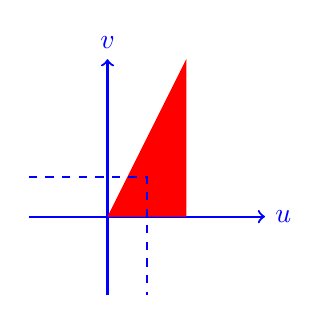
\begin{tikzpicture}
            \draw[blue, thick, ->] (-1,0) -- (2,0) node[right] {$u$};
            \draw[blue, thick, ->] (0,-1) -- (0,2) node[above] {$v$};
            \fill[red] (0,0) -- (1,0) -- (1,2);
            \draw[blue, thick, dashed](-1, 0.5) -- (0.5, 0.5) -- (0.5, -1);
        \end{tikzpicture}
    \end{subfigure}
    \hfill
    \begin{subfigure}{0.18\textwidth}
        \centering
        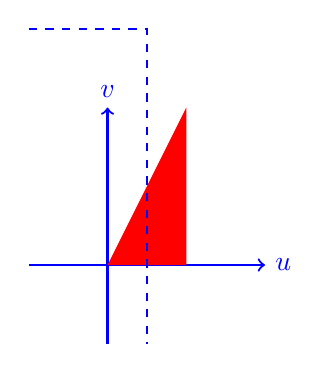
\begin{tikzpicture}
            \draw[blue, thick, ->] (-1,0) -- (2,0) node[right] {$u$};
            \draw[blue, thick, ->] (0,-1) -- (0,2) node[above] {$v$};
            \fill[red] (0,0) -- (1,0) -- (1,2);
            \draw[blue, thick, dashed] (-1, 3) -- (0.5,3) -- (0.5, -1);
        \end{tikzpicture}
    \end{subfigure}
    \hfill
    \begin{subfigure}{0.18\textwidth}
        \centering
        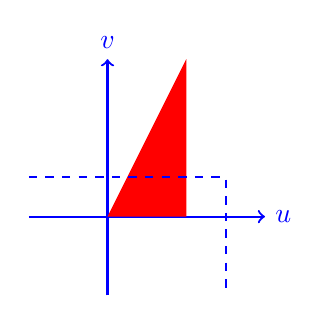
\begin{tikzpicture}
            \draw[blue, thick, ->] (-1,0) -- (2,0) node[right] {$u$};
            \draw[blue, thick, ->] (0,-1) -- (0,2) node[above] {$v$};
            \fill[red] (0,0) -- (1,0) -- (1,2);
            \draw[blue, thick, dashed] (-1, 0.5) -- (1.5, 0.5) -- (1.5,-1);
        \end{tikzpicture}
    \end{subfigure}
    \hfill
    \begin{subfigure}{0.18\textwidth}
        \centering
        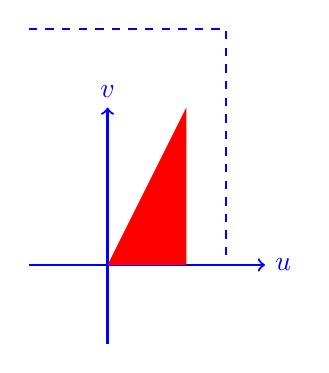
\begin{tikzpicture}
            \draw[blue, thick, ->] (-1,0) -- (2,0) node[right] {$u$};
            \draw[blue, thick, ->] (0,-1) -- (0,2) node[above] {$v$};
            \fill[red] (0,0) -- (1,0) -- (1,2);
            \draw[blue, thick, dashed] (-1, 3) -- (1.5,3) -- (1.5, 0);
        \end{tikzpicture}
    \end{subfigure}
    \label{fig:subplots}
\end{figure}
    \begin{solution}
    \item[(1)] 由定义可知$F(x,y)=\int_{-\infty}{x}\int_{-\infty}{y}f(u,v)\d u\d v$,其中x,y的可行域如下图所示,分为五个部分
    故
    \[
    F(x,y)=
    \begin{cases}
        \int_{0}^{y}\d v\int_{\frac{v}{2}}^{x}\d u, &0<x<1,0<y<2x \\
        \int_{0}^{x}\d u\int_{0}^{2u}\d v, &0<x<1, y\geq 2x \\
        \int_{0}^{y}\d v\int_{\frac{v}{2}}^{1}\d u, & x > 1, 0 < y < 2 \\
        1, & x\geq 1, y\geq 2x \\
        0, &\text{其他}
    \end{cases} = \begin{cases}
        \frac{y^2}{4}-xy, &0<x<1,0<y<2x \\
        x^2, &0<x<1, y\geq 2x \\
        y-\frac{y^2}{4}, & x > 1, 0 < y < 2 \\
        1, & x\geq 1, y\geq 2x \\
        0, &\text{其他}
    \end{cases}
    \]
    \item[(2)] 由定义可知
    \[
    f_{X}(x)=\int_{-\infty}^{+\infty}f(x,y)dy=\begin{cases}
        2x, & 0<x<1; \\
        0, & \text{其他}
    \end{cases}
    \]
    \[
    f_{Y}(y)=\int_{-\infty}^{+\infty}f(x,y)dx=\begin{cases}
        1-\frac{y}{2}, &0<y<2 \\
        0, &\text{其他}
    \end{cases}
    \]
    \item[(3)] 
    当{\color{red}0<x<1}在$X=x$的条件下,Y的条件概率密度为
    \begin{align*}
        f_{Y\mid X}(y\mid x)=\frac{f(x,y)}{f_{X}(x)}=\begin{cases}
            \frac{1}{2x}, &{\color{red}0<y<2x} \\
            0, &\text{其他}
        \end{cases}
    \end{align*}
    当{\color{red}0<y<2}在$Y=y$的条件下,X的条件概率密度为
    \begin{align*}
        f_{X\mid Y}(x\mid y)=\frac{f(x,y)}{f_{Y}(y)}=\begin{cases}
            \frac{2}{2-y}, &{\color{red}\frac{y}{2}<x<1} \\
            0, &\text{其他}
        \end{cases}
    \end{align*}
    \item [(4)]
    对于$P\left\{Y\leq \frac{1}{2}|X\leq \frac{1}{2}\right\}$可以采用条件概率公式,
    \[
    P\left\{Y\leq \frac{1}{2}|X\leq \frac{1}{2}\right\}=\frac{\iint\limits_{y\leq \frac{1}{2},x\leq\frac{1}{2}}f(x,y)\d x\d y}
    {\int_{0}^{\frac{1}{2}}f_{X}(x)\d x} =\frac{3}{4}
    \]
    而对于$P\left\{Y\leq \frac{1}{2}|X= \frac{1}{2}\right\}$则不能采用条件概率公式,因为$P\{X=\frac{1}{2}\}=0$不能做分母,此时
    就体现出来条件概率的用处
    \[
    P\left\{Y\leq \frac{1}{2}|X= \frac{1}{2}\right\}=\int_{0}^{\frac{1}{2}}f_{Y\mid X}(y\mid x)\d y
    \]
    将$X=\frac{1}{2}$带入,求出该条件概率为$\frac{1}{2}$ 
    \item [(5)]
    方法一:分布函数法 \\
    \begin{center}
        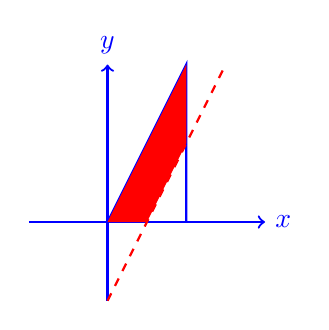
\begin{tikzpicture}
            \draw[blue, thick, ->] (-1,0) -- (2,0) node[right] {$x$};
            \draw[blue, thick, ->] (0,-1) -- (0,2) node[above] {$y$};
            \draw[blue, thick] (0,0) -- (1,2) -- (1,0);
            \draw[red, thick, dashed] (0, -1) -- (0.5, 0) -- (1.5,2); 
            \fill[red](0,0)--(0.5,0)--(1,1)--(1,2)--(0,0);
        \end{tikzpicture}
    \end{center}
    $F_{Z}(z)=P\{2X-Y\geq Z\}=\iint\limits_{2x-y\leq z}f(x,y)\d x\d y$ ,绘制$y\geq 2x-z$,讨论截距,如图所示,其结果如下
    \[
    F_{Z}(z) = \begin{cases}
        0, & z < 0 \\
        z-\frac{z^2}{4}, & 0\leq z < 2 \\
        1, & z\geq 2
    \end{cases}
    \]
    方法二:卷积公式 \\
    由卷积公式有$f_Z(z)=-\int_{-\infty}^{+\infty}f(x,2x-z)dx$,此时把$f(x,y)$中的y全部转换为$z$并确定$z$的取值范围
    即\[f(x,2x-z)=\begin{cases}
        1, &0<x<1, 0<2x-z<2x\implies, 0<x<1, 0<z<2x \\
        0, &\text{其他}
    \end{cases}
    \]
    此时再对$x$进行偏积分即可,绘制$x-z$图像,首先确认z的范围,再从z上对x进行积分
    \begin{center}
        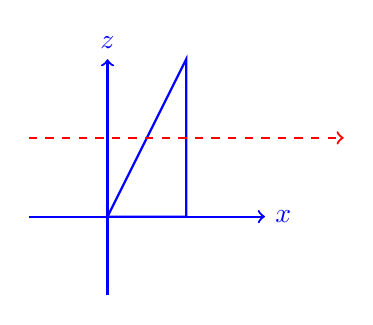
\begin{tikzpicture}
            \draw[blue, thick, ->] (-1,0) -- (2,0) node[right] {$x$};
            \draw[blue, thick, ->] (0,-1) -- (0,2) node[above] {$z$};
            \draw[blue,thick](0,0)--(1,0)--(1,2)--(0,0);
            \draw[red,thick,->, dashed](-1,1)--(3,1);
        \end{tikzpicture}
    \end{center}
    如图,最终
    \[
    f_{Z}(z)=\begin{cases}
        1-\frac{z}{2}, &0\leq z < 2;\\
        0, &其他
    \end{cases}
    \]
    \end{solution}
\end{enumerate}

\section{求一离散一连续随机变量函数的分布}

\begin{enumerate}[label=\arabic*.,start=10]
    % 例题3.10
    \item  (2020,数一)设随机变量$X_1,X_2,X_3$相互独立,$X_1$与$X_2$均服从标准正态分布,$X_3$的概率分布为$P\{X_3=0\}=P\{X_3=1\}=\frac{1}{2}$,$Y=X_3X_1+(1-X_3)X_2$。
    \begin{enumerate}
        \item [(1)] 求$(X_1,Y)$的联合分布函数(结果用标准正态分布函数$\Phi(x)$表示);
        \item [(2)] 证明$Y$服从标准正态分布.
    \end{enumerate}
    
    \begin{solution}
    一离散加一连续的基本方法就是"全概率公式+独立性"
    \item [(1)]
    \begin{align*}
        F(X_1,Y)&=P\{X\leq x, Y\leq y\} \\
        &=P\{X_1\leq x, X_3X_1+(1-X_3)X_2\leq y\} \\
        &\xlongequal{\text{全概率公式}}P\{X_1\leq x, X_2\leq y, X_3=0\} + P\{X_1\leq x, X_1\leq y, X_3=1\} \\
        &\xlongequal{\text{独立性}}P\{X_1\leq x\}P\{X_2\leq y\}\frac{1}{2} + \frac{1}{2}P\{X_1\leq \min{(x,y)}\} \\
        &=\frac{1}{2}\Phi(x)\Phi(y)+\frac{1}{2}\Phi(\min{(x,y)})
    \end{align*}
    \item [(2)]
    方法一,通过Y的分布函数确定
    \begin{align*}
        F_{Y}(y)=P\{Y\leq y\} &=P\{X_3X_1+(1-X_3)X_2\leq y\} \\
        &= (\text{和(1)完全一致省去})\ldots \\
        &= \Phi(y)
    \end{align*}
    方法二,直接求边缘分布函数
    \begin{align*}
        F_{X}(x) &=P\{X\leq x\}=F(X,+\infty) \\
        F_{Y}(y) &=P\{Y\leq y\}=F(+\infty,Y) \\
        F_Y(y) &= F(\infty, y) = \frac{1}{2}\Phi(y)+\frac{1}{2}\Phi(y) = \Phi(y)
    \end{align*}
    故$Y\sim N(0,1)$
    \end{solution}
\end{enumerate}

\ifx\allfiles\undefined
\end{document}
\fi